% Definition der Klasse des Dokumentes
\documentclass[11pt, a4paper]{article}

\usepackage[T1]{fontenc}        % Sorgt u.a. dafür, dass Texte vernünftig markierbar werden auch bei Sonderzeichen
\usepackage{ae,aecompl} %bessere Schrift
\usepackage{gensymb}
\usepackage[ngerman]{babel}     % Deutsches Wörterbuch usw.
\usepackage{epstopdf}   % Wandelt .eps Dateien automatisch um
\usepackage{url}    % für URL mit \url{.....}
\usepackage[font=small,labelfont=bf]{caption}       % Optionen für Bild- und Codeunterschriften
\usepackage[hidelinks]{hyperref}                    % damit Links in der PDF anklickbar werden
\usepackage{booktabs}   % bessere Tabellen mit Abstand zur hline
\pagenumbering{arabic}
\usepackage[babel,german=guillemets]{csquotes} %deutsches Anführungszeichen
\usepackage{float} %bessere Positionierungsoptionen

% Standardpakete für deutsche Sprache
\usepackage[utf8]{inputenc}
\usepackage[ngerman]{babel}

% Volle Seite nutzen
\usepackage{fullpage} 
\headsep 1cm
\parindent 0cm

% einige Pakete für Mathematische Darstellung
\usepackage{amssymb, amstext, amsmath}
\usepackage{fancyhdr}

% ein Paket für die Zählung von Seiten
\usepackage{count1to}
\usepackage{lastpage} 

%Paket für Aufzählungsbuchstaben
\usepackage{enumitem}

\usepackage{nameref}



% HIER DIE NAMEN UND EMAIL ANPASSEN
\def \ATutantName{Moritz Breipohl}
\def \ATutantEmail{mbreipohl@techfak.uni-bielefeld.de}
\def \BTutantName{Markus Rothgänger}
\def \BTutantEmail{mrothgaenger@techfak.uni-bielefeld.de}
% HIER DIE VERSUCHSNUMMER ANPASSEN
\def \Versuchsnummer{Versuch 5}
% HIER DIE GRUPPENNUMMER ANPASSEN
\def \Gruppennummer{Gruppe 5}
% HIER DEN TUTORNAMEN ANPASSEN
\def \Tutorname{Lukas Schmidt, Robin Ewers}

% Kopfzeile und Fußzeile
\lhead{\Versuchsnummer}
\chead{\textbf{Digitalelektronisches Praktikum}}
\rhead{\today}
\lfoot{\Gruppennummer}
\rfoot{\thepage\ von \pageref{LastPage}}
\cfoot{}

% Wird zur Einbindung von Bildern benötigt
\usepackage{graphicx}
\graphicspath{{images/}}

% Physikalische Einheiten darstellen
\usepackage{siunitx}

% Einbinden des Literaturverzeichnisses
\usepackage[style=numeric-comp]{biblatex}
\bibliography{literatur.bib}

% Wird zum Einbinden von LaTeX Code benötigt
\usepackage{color}
\usepackage{showexpl}
\lstset
{
    language=[LaTeX]TeX,
    breaklines=true,
    basicstyle=\tt\scriptsize,
    keywordstyle=\color{blue},
    identifierstyle=\color{magenta},
}

\renewcommand{\footrulewidth}{0.4pt}
\pagestyle{fancy}

% Konfiguration des Deckblatts
\begin{titlepage}
\title{\textbf{Digitalelektronisches Praktikum\\ Versuch 5}}
\author{\ATutantName \\ \emph{\ATutantEmail} \and \BTutantName\\ \emph{\BTutantEmail}}
\date{\Gruppennummer \\[3ex] Tutor: \Tutorname \\[3ex] \today}
\end{titlepage}

\begin{document}
% Einfügen des Deckblatts
\clearpage
\maketitle
\thispagestyle{empty}
\newpage

%%%%%%%%%%%%%%%%%%%%%%%%%%%%%%%%%%%%%%%%%
%%% Ab hier Beginn des Laborberichts: %%%%%%%%%%%%%%%%%%%%%

\section*{Versuchsaufbau}
\subsection*{Aufgabe}
Im fünften Versuch sollten zwei verschiedene CMOS-Logikgatter mit mindestens zwei Eingängen sowohl simuliert als auch auf dem Steckbrett aufgebaut werden. Zur Untersuchung der Schaltung sollte das erwartete Verhalten anhand einer Logiktabelle mit dem gemessenen Verhalten verglichen werden. Des weiteren sollte die Schaltung durch eine integrierte Schaltung realisiert werden. Schließlich sollten alle Schaltungen auf ihre Verzögerungszeit und die Stromaufnahme untersucht werden.
\subsection*{Erwartung}
Die generelle Erwartung ist, dass alle Gatter-Aufbauten ein gleiches Logikverhalten aufweisen. Aus den letzten Versuchen abgeleitet ist eine teils hohe Abweichung zwischen realen und simulierten Messungen in Bezug auf die Verzögerungszeit und die Stromaufnahme zu erwarten. Dennoch ist auch eine Abweichung der Messwerte von integriertem Schaltkreis (auch IC (integrated Circuit)) und dem aus Transistoren aufgebauten Gatter möglich.

% Die Logikformeln sind jetzt in den Tabellen der Messwerte integriert

\subsection*{Aufbau}
Es wurden ein NAND- und ein NOR-Gatter untersucht. Beide Aufbauten sind für den Simulator und das Steckbrett identisch.
Zu beachten ist, dass die Messpunkte für die Ausgangsspannung ($U_{OUT}$) und den statischen Querstrom ($I_{quer}$) in den Schemata eingezeichnet sind. Hier wurden dann Multimeter Spannungs- bzw. Stromrichtig angeschlossen.
Der Aufbau des NAND-Gatters ist in \autoref{aufbauNAND} dargestellt, der des NOR-Gatters in \autoref{aufbauNOR}. Die beiden Eingangsspannungen ($U_{IN1}$ und $U_{IN2}$) wurden zeitweise über entprellte Taster, sowie über den Funktionsgenerator bedient.
Zur Messung der Verzögerungszeit wurde außerdem die Ausgangsspannung $U_{OUT}$ mithilfe des Oszilloskopes betrachtet.
Mit gleicher Handhabung zum Messen wurden die Schaltungen mit Hilfe von ICs aufgebaut. Diese Aufbauten am Steckbrett sind in \autoref{aufbauNANDIC} (NAND) und \autoref{aufbauNORIC} (NOR) zu sehen.
\begin{figure}[htb]
    \centering
    \begin{minipage}[t]{0.45\linewidth}
        \centering
        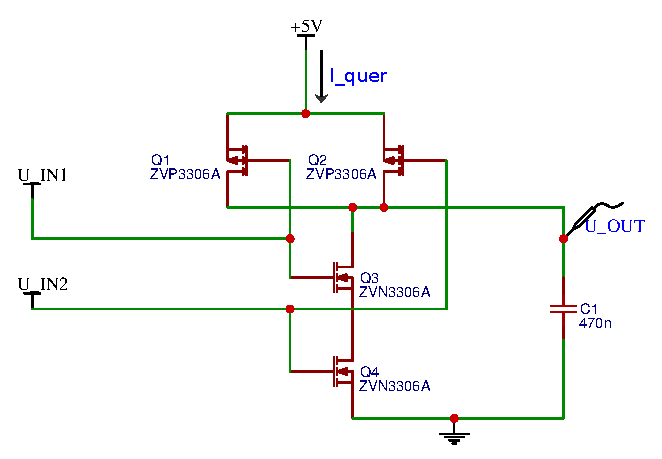
\includegraphics[width=\linewidth]{NAND.pdf}
        \caption{Aufbau des NAND-Gatters}
        \label{aufbauNAND}
    \end{minipage}% 
    \hfill
    \begin{minipage}[t]{0.45\linewidth}
        \centering
        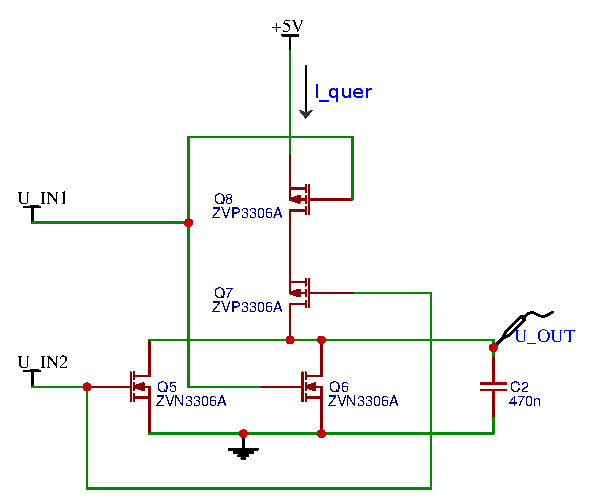
\includegraphics[width=\linewidth]{NOR.pdf}
        \caption{Aufbau des NOR-Gatters}
        \label{aufbauNOR}
    \end{minipage}
\end{figure}
\begin{figure}[htb]
    \centering
    \begin{minipage}[t]{0.45\linewidth}
        \centering
        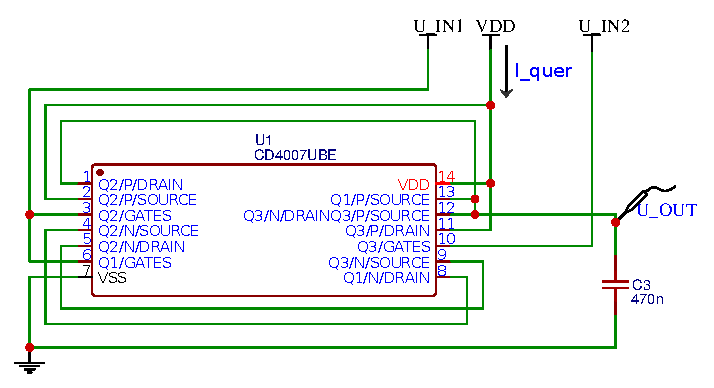
\includegraphics[width=\linewidth]{IC_NAND.pdf}
        \caption{Aufbau des NAND-Gatters mit IC}
        \label{aufbauNANDIC}
    \end{minipage}% 
    \hfill
    \begin{minipage}[t]{0.45\linewidth}
        \centering
        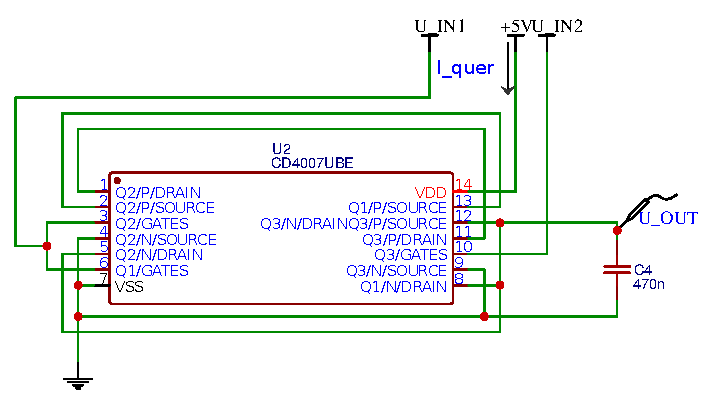
\includegraphics[width=\linewidth]{IC_NOR.pdf}
        \caption{Aufbau des NOR-Gatters mit IC}
        \label{aufbauNORIC}
    \end{minipage}
\end{figure}
\subsection*{Verwendete Bauteile}
Multimeter, ein Strombegrenztes Versorgungsnetzteil mit einer konstanten Spannung von $5V$, jweils zwei Transistoren vom Typ \textit{ZVN3306a} sowie vom Typ \textit{ZVP3306a}, ein Kondensator mit einer Kapazität von $470nF$, Funktionsgenerator und Oszilloskop, IC vom Typ \textit{CD4007UB}.

\section*{Durchführung}

\subsection*{Verifizierung des Logikverhaltens}

Die Auswirkungen jeder Eingangskombination auf die Ausgangsspannung wurde hier geprüft. Dabei wurden die Eingäng über entprellte Schalter angesteuert, welche an einem Netzteil mit 5V Versorgungsspannung angeschlossen waren. Am Ausgang der Schaltung befand sich eine LED, über deren Status (leuchtet oder leuchtet nicht) geprüft werden konnte, ob die Schaltung den Stromfluss zum Ausgang erlaubt. Ein Leuchten der LED wurde mit einer 1 eingetragen, ein nicht-Leuchten mit einer 0.

\subsection*{Messung des statischen Querstroms}

Zur Messung des Querstroms wurde am Steckbrett ein Amperemeter in Reihe in den Versorgungsstromkreis geschaltet.
Die Versorgungsspannung lag bei konstanten $U_{VDD} = 5V$ mit einer Strombegrenzung von etwa $I = 0.2A$. Es war darauf zu achten, dass während der Strommessung kein Schaltvorgang durchgeführt wurde, da sonst der dynamische statt dem statischen Querstrom gemessen würde.
In der Simulation wurde die Stromaufnahme an der Spannungsquelle gemessen. 

\subsection*{Messung der Verzögerungszeit}

Am Steckbrett wurde das Oszilloskop genutzt, um einen oder beide Eingänge mit einer vom Funktionsgenerator generierten Kurve zu versorgen. Die Eingangskurve sowie der Spannungsverlauf am Ausgang wurden vom Oszilloskop aufgenommen und die Verzögerungszeit für die steigende als auch die abfallende Flanke mithilfe der Cursor bestimmt. \\

Ähnlich wurde die Verzögerungszeit in der Simulation bestimmt. Die beiden Eingänge wurden als pulsierende Spannungsquellen definiert, die eine unterschiedlichen Rythmus [DER SATZ HÖRT HIER AUF :D]

\section*{Messergebnisse}
\subsection*{Logikverhalten}


\begin{table}[H]
	\center
	\begin{tabular}{c|c||c||c|c|c}
	Input A 	& Input B 	& Erwartetes Ergebnis 	& eigene Schaltung & IC & Simulation	\\ \hline
	0 & 0 & 1 & 1 & 1 & 1		\\
	0 & 1 & 0 & 0 & 0 & 0		\\
	1 & 0 & 0 & 0 & 0 & 0		\\
	1 & 1 & 0 & 0 & 0 & 0		\\
	\end{tabular}
	\caption{Logikverhalten der NOR Gatter}
	\label{logikNOR}


	\center
	\begin{tabular}{c|c||c||c|c|c}
	Input A 	& Input B 	& Erwartetes Ergebnis 	& eigene Schaltung & IC & Simulation	\\ \hline
	0 & 0 & 1 & 1 & 1 & 1		\\
	0 & 1 & 1 & 1 & 1 & 1		\\
	1 & 0 & 1 & 1 & 1 & 1		\\
	1 & 1 & 0 & 0 & 0 & 0		\\
	\end{tabular}
	\caption{Logikverhalten der NAND Gatter}
	\label{logikNAND}
\end{table}

\subsection*{Querströme}

\begin{table}[H]
	\center
	\begin{tabular}{c|c}
	& Querstrom [\si{\micro\ampere}]	\\ \hline
	Selbstgbaut & $5.06$ 		\\
	IC 			& $224.6$ 		\\
	Simulation 	& $0$\\
	\end{tabular}
	\caption{statischer Querstrom an den NOR Gattern}
	\label{querstromNAND}


	\center
	\begin{tabular}{c|c}
	& Querstrom [\si{\micro\ampere}]	\\ \hline
	Selbstgbaut & $260$ 		\\
	IC 			& $60$ 			\\
	Simulation 	& $0$\\
	\end{tabular}
	\caption{statischer Querstrom an den NAND Gattern}
	\label{querstromNAND}
\end{table}

\begin{figure}[H]
    \centering
    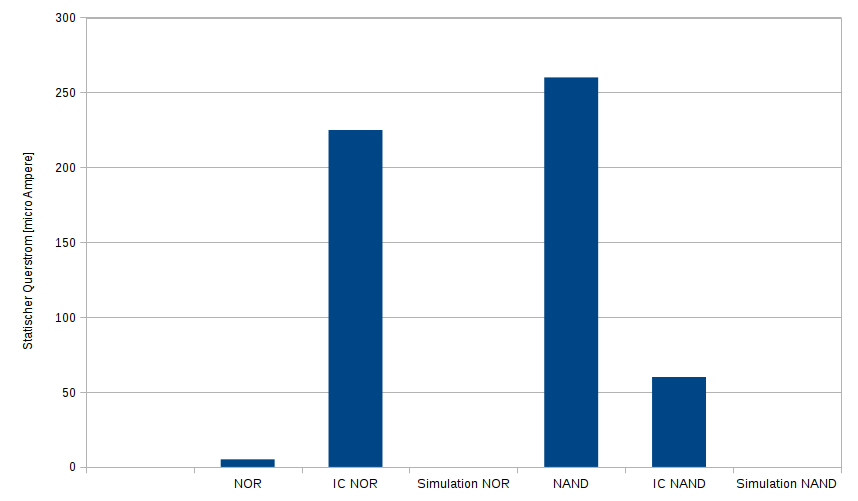
\includegraphics[width=\linewidth]{images/querstrom.png}
    \caption{Querströme}
    \label{graphQuerstrom}
\end{figure}


\subsection*{Verzögerungszeiten}
Da die Verzögerungszeiten für beide Eingänge sehr ähnlich bzw. gleich waren, werden hier der Übersicht halber nur die Messergebnisse für die Veränderung des Zustands eines Eingangs aufgezeigt.

\begin{table}[H]
	\center
	\begin{tabular}{c|c|c}
	& Flanke steigend [\si{\micro}S] & Flanke fallend [\si{\micro}S] 	\\ \hline
	Selbstgbaut & $2.9$ 	& $19.6$	\\
	IC 			& $232$ 	& $1520$	\\
	Simulation 	& $4.98$		& $39.05$\\
	\end{tabular}
	\caption{Verzögerungszeiten an den NOR Gattern}
	\label{verzögerungszeitenNOR}



	\center
	\begin{tabular}{c|c|c}
	& Flanke steigend [\si{\micro}S] & Flanke fallend [\si{\micro}S] 	\\ \hline
	Selbstgbaut & $5.6$ 	& $7.9$	\\
	IC 			& $710$ 	& $130$	\\
	Simulation 	& $8.94$		& $11.93$\\
	\end{tabular}
	\caption{Verzögerungszeiten an den NAND Gattern}
	\label{verzögerungszeitenNAND}
\end{table}

\begin{figure}[H]
    \centering
    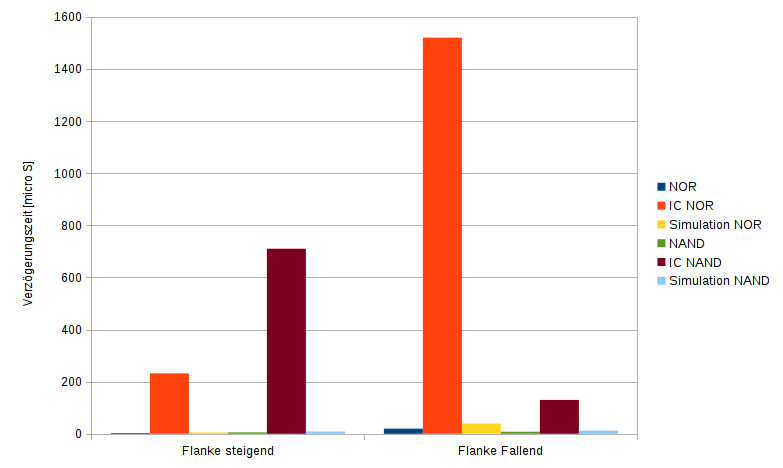
\includegraphics[width=\linewidth]{images/verzoegerungen.png}
    \caption{Verzögerungszeiten}
    \label{graphVerzögerungen}
\end{figure}

\section*{Beobachtungen}
Da die Ausgangswerte für alle Aufbauten mit den erwarteten Werten übereinstimmen (siehe \autoref{logikNOR} und \autoref{logikNAND}, können wir uns sicher sein, dass wir die Schaltungen korrekt aufgebaut haben

Anhand von \autoref{graphQuerstrom} stellt man fest, dass in der Simulation keinerlei Querstrom abfällt. Da wir hier mit einer idealisierten Schaltung ohne implizite Widerstände arbeiten, ist dies auch nicht weiter verweunderlich.
Dahingegen ist allerdings der große Unterschied zwischen dem selbstgebauten NOR- und NAND-Gatter auszumachen. Besonders interessant ist dazu das entgegengestzte Verhalten des ICs: Das integrierte NOR hat eine deutlich höhere Stromaufnahme als das integrierte NAND.
\\
Erkennbar an \autoref{graphVerzögerungen}, stechen die Verzögerungszeiten der integrierten Schaltungen besonders heraus und liegen bis zu 76 Mal höher als bei der selbstgebauten Schaltung. Zudem fällt auf, dass die fallende Flanke an allen NOR Gattern etwas stärker verzögert ist als in den anderen Fällen.

\section*{Auswertung}
Überraschend ist der große Unterschied zwichen Stromaufnahme des NORs und des NANDs, da beide die gleichen Bauteile verwenden, nur in einer anderen Konfiguration. Bei genauerer Überlegung kommt man jedoch zu dem Schuss, dass aufgrund der Tatsache, dass die Schaltungen unterschiedliche Ergebnisse erzielen auch unterschiedliche interne Zustände besitzen. Kurz gesagt: Das NAND hat eine höhere Stromaufnahme, da im statischen Zustand mehr Transistoren angesprochen werden als beim NOR. Daraus folgt dann auch der höhrere statische Querstrom. Im Gegensatz dazu steht jetzt allerdings das IC. Hier kann nur vermutet werden, dass aufgrund der internen Schaltung das NAND etwas simpler ist als das NOR und dementsprechend auch einen geringeren Querstrom aufzeigt.
\\
\\
Die deutlich langsamere Schaltzeit der ICs erklärt sich dadurch, dass die ICs Bausteine mit vielen verschiedenen Funktionen sind und dementsprechend auch mehr Transistoren besitzen, welche die Schaltzeit negativ beeinflussen.
Die Steckbrettschaltung sowie die Simulation liegen hingegen sehr nah beieinander, wobei die Verzögerungszeit auf dem Steckbrett etwas geringer ist als die simulierte. Da die Bauteile alle eine gewisse Fehlertoleranz haben, werden identische Schaltungen mit unterschiedlichen Transistoren gleicher Baureihe unterschiedliche Ergebnisse erzielen. Die im LTSpice verwendeten Transistoren halten sich dabei an den vom Hersteller garantierten Wert und schalten dementsprechend ein wenig langsamer.
\\
Hieraus lässt sich entnehmen, dass für eine besonders kurze Verzögerung eine dedizierte Schaltung besser geeignet ist, als ein Multifunktionsbaustein, welcher dann auf eine bestimmte Funktion beschränkt wird.


[ERWARTUNGEN? Blub, habe keine Ahnung]

\end{document}